\section*{\color{SectionBlue}{Background Information}} \label{sec:sections}
\addcontentsline{toc}{section}{Background Information}
\subsection*{\color{SubSectionBlue}{A Technological World}}
\addcontentsline{toc}{subsection}{A Technological World} \\
Technology is a powerful agent of change that has shifted the focus of corporations and individuals from face-to-face interactions to online communication. Web applications deployed on accessible backend services such as Heroku or AWS can link family members who live in different parts of the world or companies trying to reach an international consumer base. On top of that, in the public sector, shared hospital networks (usually hosted on cloud services) can help doctors receive real-time electronic health records. The comprehensive streaming of data present in most hospitals can improve their ability to take action regarding critical patient data. 

\vspace{1mm}

Simply put, technology represents convenience and accessibility in the eyes of individuals, and humans have incorporated this new tool into most aspects of their lives. For example, in the United States alone, Internet traffic for banks grew by 77.6\% between July 2000 and July 2001 \cite{mia_e-banking_2007}. On top of that, online retail sales have increased to 269 billion USD in 2004 from a mere 45 billion USD in 2000 \cite{rohm_typology_2004}. Finally, since the healthcare industry is under constant pressure to reduce costs and improve patient care, information technology can help a hospital manage risks and improve organizational performance \cite{bradley_empirical_2012}. Technology such as computer tomography (CT) scanners and X-ray machines help doctors identify issues much faster. So, in the 21st century, hospitals and businesses alike have seen a growth in users, highlighting the ever growing impact of technology.

\subsection*{\color{SubSectionBlue}{The Dangers of Cyberspace}}
\addcontentsline{toc}{subsection}{The Dangers of Cyberspace} \\

The recent emergence of this online world has been accompanied by increasing attacks on firms and hospitals. However, the reality is that company databases are not secure enough to handle the complexity of the Trojans deployed. In 2015, Chinese hackers stole the background information of 21.5 million federal employee's and 5.6 million fingerprints -- credentials that were needed for identity theft. Since the Office of Personnel Management was unaware of this breach, every American who had a background check in the last 15 years was affected \cite{gootman_opm_2016}. This attack suggests that databases are not strong enough to keep important information secure. Breaches in security happen way too often and the information of 44 million consumers is dangled in the air \cite{rachwald_is_2008}. 
\vspace{1mm}

The impact of cyber attacks expands far beyond stolen social security numbers and bank account information. The majority of damage occurs when hospital systems are infiltrated in an attempt to confiscate electronic health records -- a valuable commodity on the black market. Hacker groups have the potential to disable CT scanners and other technological necessities, placing human lives in serious danger. However, an attacker with access to medical records can do much more than simply sell it on the black market or hold it for ransom. As Israeli researchers Mirsky et al. \cite{mirsky_ct-gan_2019} first proposed, deep learning can be used to add or remove the evidence of medical conditions from volumetric (3D) medical scans \cite{mirsky_ct-gan_2019}. So, to understand the potential danger of existing malware, they infiltrated a local hospital, intercepted CT scans, and altered the images [Fig 1]. 

\begin{figure}[ht]%
    \centering
    \subfloat[Original CT Scan]{{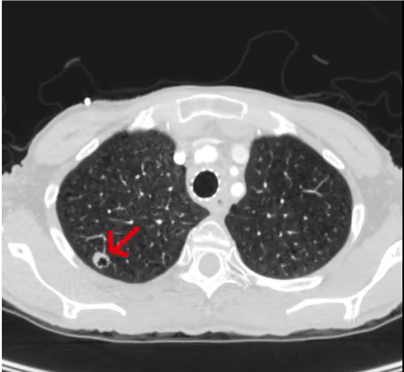
\includegraphics[width=5cm]{Images/ct-scan-orig.png} }}%
    \qquad
    \subfloat[Altered CT Scan]{{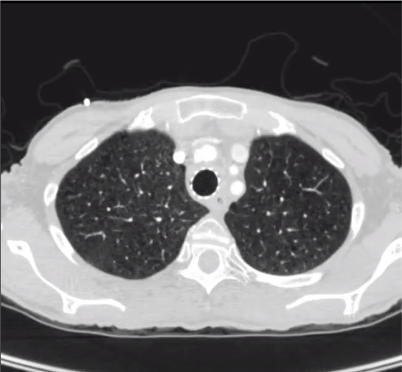
\includegraphics[width=5cm]{Images/ct-scan-alter.png} }}%
    \caption{Modification on CT Scans by Mirsky et al. \cite{mirsky_ct-gan_2019}}%
    \label{fig:example}%
\end{figure}
\addcontentsline{toc}{subsubsection}{Figure 1: Altered CT Scans} \\

By training a generative adversarial network on 888 CT scans, the images were successfully altered with deep learning. The effectiveness of the attack was then verified in a blind and open trial where radiologists were asked to diagnose complete CT scans. In general, the attack had an average success rate of 99.2\% for cancer insertion and a 95.8\% for cancer removal \cite{mirsky_ct-gan_2019}. This newfound application of malware places thousands of lives in danger and emphasizes the far-reaching repercussions of cyber attacks.

\subsection*{\color{SubSectionBlue}{Two Targets}}
\addcontentsline{toc}{subsection}{Two Targets} \\

When looking at the targets of these cyber attacks, there are two major firm-types present: bigger targets and small-medium targets. Bigger targets are firms that have a constant influx of money from the government and have substantial changes to their budget each year. Bigger targets can also include cybersecurity departments that receive a large portion of the firm’s budget and don’t have an immediate limit on monetary spending. On the other hand, small-medium targets, like their name suggests, are smaller firms that are heavily-restricted with the available funding for cyber security, generally working with a fixed budget \cite{fielder_decision_2016}. They can also include cybersecurity departments that receive a small portion of the firm’s budget and face immediate restrictions. This smaller budget forces trade-offs within the company where the chief technical officer has to make important decisions. The bigger targets have layers of security protecting the information making it more secure when compared to a smaller target that does not have the resources to implement that software. For this reason, approximately 72\% of cyber breaches occur at Small-Medium targets making the information more insecure when compared to bigger firms \cite{fielder_decision_2016}.  
\vspace{1mm}

However, smaller targets do provide substantial benefits to their customers despite their decrease in size. Due to the research and development nature of small-medium targets, they are likely to have more classified data when compared to bigger targets, who are trusted with more public data. On top of that, facilities like hospitals spend so much of their budget on equipment and staffing that little money gets allocated towards infrastructure development. The lack of funding increases the vulnerability of electronic health records. Since the data is more valuable, if there is a breach in a small-medium target, the risks are significantly higher when compared to a breach in a larger company. So, it is important for small-medium targets to implement controls that can mitigate vulnerabilities present in the system. Despite the importance of these controls, most Chief Information Security Officers (CISO) are not confident in patching up vulnerabilities under the budget constraint that is present in the company. For example, in a report published by Deloitte and NAISCO, 75.5\% of CISO’s cited a lack of sufficient budget as the top challenge (Fielder, 2016). Also, the study finds that 49\% of cybersecurity firms only have 6 to 15 specialists working to protect the data. 

\begin{figure}[ht]%
\centering
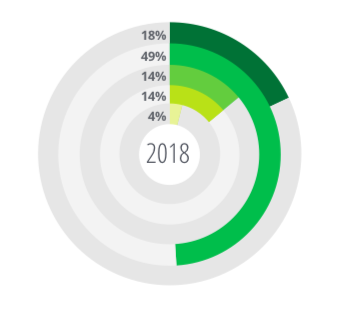
\includegraphics[width=5cm,height=5cm]{Images/expertise.png}
\caption{Top Restriction for Small Targets \cite{noauthor_deloitte_nodate}}%
\end{figure}
\addcontentsline{toc}{subsubsection}{Figure 2: Top Restriction for Small Targets} 

Each color in the chart [Fig 2] signifies a range of cybersecurity specialists . From the top (18\%) to the bottom (4\%), the first bar (18\%) represents 1-5 full-time employees, the second bar (49\%) represents 6-15 full-time employees, the third bar (14\%) represents 16-25 full-time employees, the fourth and last bar (4\%) represents 26-50 full-time employees. Since there is an abundant shortage of specialists in this field, action needs to be taken. For this reason, it is important to develop a system that will analyze the trade-offs of each control and advise the implementation of the controls that offer the greatest mitigation against an attack. 

\subsection*{\color{SubSectionBlue}{Endpoint Protection Data}}
\addcontentsline{toc}{subsection}{Endpoint Protection Data} \\

In an attempt to combat this growing issue, third-party organizations, like KnowBe4, publish statistics on the specifics of each attack in Endpoint Protection Reports. The Endpoint Protection Report provides information regarding the frequency of cyber attacks in a given year and the effectiveness of potential countermeasures which companies might implement to protect themselves. Using the 2009 endpoint protection report on security breaches and cost of downtime, Rakes et al. \cite{rakes_it_2012} from the Pamplin College of Business developed a dataset which consolidated the information in the report \cite{rakes_it_2012}. Qualitative attributes present in the endpoint protection report, such as countermeasure effectiveness, were expanded into quantitative values such as survival probabilities. The dataset expresses the relationships between a variety of different threats and countermeasures.

\begin{figure}[ht]%
\centering
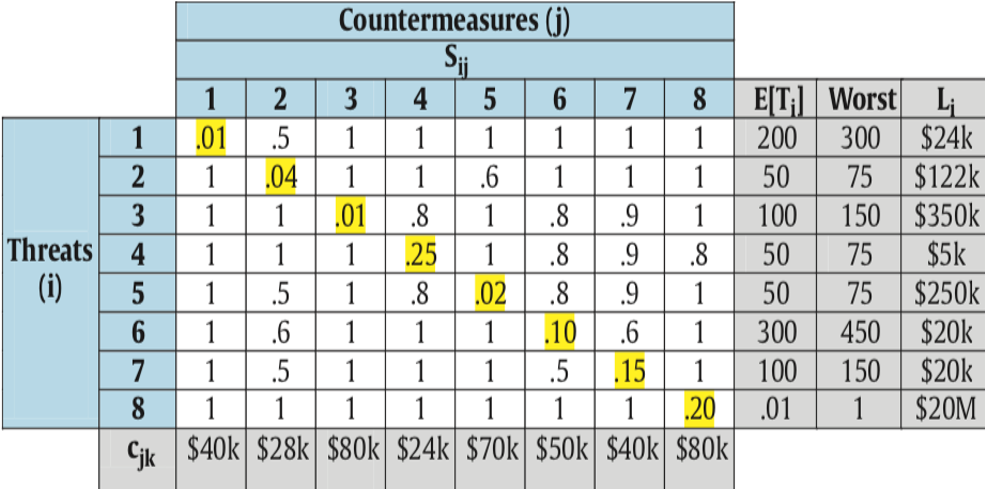
\includegraphics[width=15cm,height=5.15cm]{Images/protection-data.png}
\caption{Compiled Cybersecurity Data by Rakes et al. \cite{rakes_it_2012}}%
\end{figure}
\addcontentsline{toc}{subsubsection}{Figure 3: Compiled Cybersecurity Data} 

When analyzing the data set [Fig 3] compiled by Rakes et al. \cite{rakes_it_2012}, there are three major aspects that are taken into consideration: the survival probabilities, the general attack statistics, and the cost of implementing the countermeasures. The survival probabilities, which is the array in white, represent the probability, $P(X, Y)$, of an attack (X) succeeding when a certain countermeasure (Y) is implemented. Although all countermeasures are most effective against a specific threat, the array has off-diagonal terms because some countermeasures work not only against their primary threat, but because they provide additional protection against other threats as well. The general attack statistics, which are the three gray-shaded columns, represents the expected number of attacks in a given year ($E[T_i]$), the worst-case number of attacks in a given year ($W[T_i]$), and the damage incurred from each successful attack ($L_i$). Finally, the cost of implementing the countermeasures, the gray-shaded row, represents the monetary cost a company would have to pay in order to install that specific countermeasure. 

\subsection*{\color{SubSectionBlue}{Linear Optimization Model}}
\addcontentsline{toc}{subsection}{Linear Optimization Model} \\

Using this compiled data set, Rakes et al. \cite{rakes_it_2012} developed a linear optimization model that attempted to allocate budgets for companies of all sizes. The model selected countermeasures based upon quantitative factors such as threat levels and countermeasure effectiveness \cite{rakes_it_2012}.  The model took in the budget of a company as the input and attempted to choose appropriate countermeasures to protect that firm. Depending on the countermeasures chosen, the model would output the expected damage to the company in the case of an attack. In order to simulate the decision making process of firms, Rakes et al. followed three major steps. The first involved determining the probability $P_i$ that a threat $i$ would cause monetary loss.

\begin{equation}
P_i = \prod(1 - Y_i e_{ij}) 
\end{equation}

However, in order to linearize the model, the effectiveness, $e_{ij}$, was replaced with the proportion of threats that will survive an attack. On top of that, constraints were added to ensure that the proportion of threats which survived the first countermeasure would be assigned to the second countermeasure (Rakes, 2010). The process repeated for all countermeasures in which the binary selector, $Y_i$, was true. After the assignment process, the model estimated the damage to a company by surviving threats. The monetary loss (both explicit and implicit) was calculated by multiplying the number of surviving attacks by the loss per successful attack. This allowed Rakes et al. to approximate the amount of money saved by implementing each countermeasure. Once calculating the monetary loss, the model ensured that the cost of implementing the countermeasures would remain under a specified budget. 
\vspace{1mm}

Using the compiled data set [Fig 3], Rakes et al. \cite{rakes_it_2012} tested their linear optimization model on both the expected-case attacks and the worst-case attacks. The researchers looked at the relationship between company budget and monetary loss in the case of an attack. The loss was used as an indirect measure of the algorithm’s decision making capabilities. The monetary loss was predicted at each of 16 different budgets, comprising bigger and small-medium targets \cite{rakes_it_2012}.

\begin{figure}[ht]%
\centering
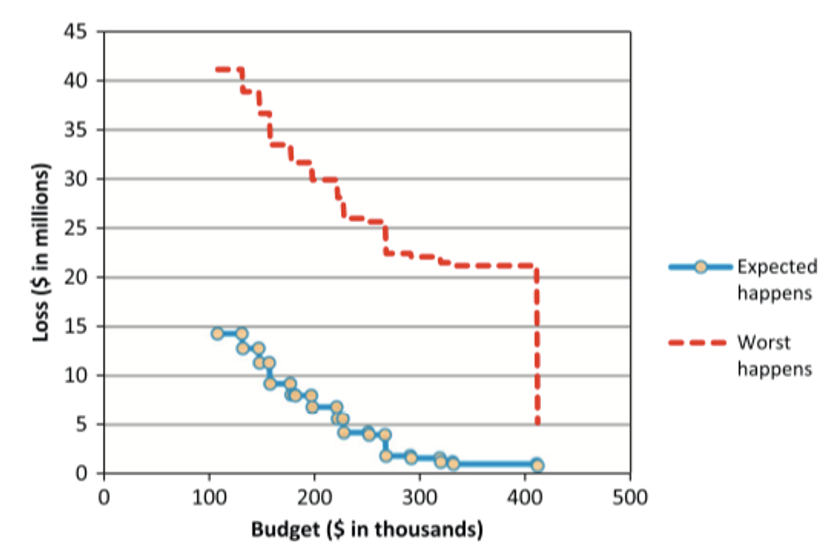
\includegraphics[width=9cm,height=6.5cm]{Images/linear-optimization.png}
\caption{Model Allocation at Each Budget Range \cite{rakes_it_2012}}%
\end{figure}
\addcontentsline{toc}{subsubsection}{Figure 4: Model Results}

When analyzing both the expected-case relationships and worst-case relationships of the linear model [Fig. 4], the budget and monetary loss seem to have an inverse relationship. With a higher budget, the algorithm can implement more countermeasures and the monetary loss faced by the companies is reduced. However, with small-medium targets, the linear optimization model predicts a high monetary loss in the case of an attack. So, an algorithm is needed that can help small-medium targets effectively allocate their cybersecurity budgets since it is these smaller targets that are more susceptible to malware.

\subsection*{\color{SubSectionBlue}{Knapsack Problem}}
\addcontentsline{toc}{subsection}{Knapsack Problem} \\

To improve the budget allocation of small-medium targets, the budget allocation problem has to be analyzed from a different angle. In fact, the complex trade-offs caused by a budget constraint can be simplified to a single-choice Knapsack problem. The knapsack problem is a NP-Complete optimization problem with the goal of finding, in a set of items with given values and weights, the subset of items with the highest total value, under a weight restriction \cite{murawski_how_2016}.

\begin{figure}[ht]%
\centering
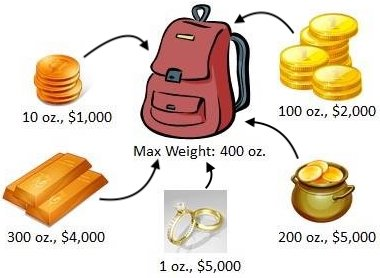
\includegraphics[width=5cm,height=5cm]{Images/knapsack-graphic.jpeg}
\caption{Knapsack Problem \cite{pan_comparison_2018}}%
\end{figure}
\addcontentsline{toc}{subsubsection}{Figure 5: Problem Explanation}

In this problem, a value has to be optimized while remaining under a certain constraint. A common interpretation of the knapsack problem is to design a system that can handle a large influx of data while remaining under corporate budget. Other interpretations include determining which parts to purchase in order to increase the fuel efficiency of a car. In the case of cyber security budget allocation, the mitigation of an attack has to be maximized while remaining under the budget constraint provided to the cybersecurity department of the small-medium target. Computer scientists have successfully solved this Knapsack problem classically; however, the algorithms are generally slow and time-consuming. With quantum computers providing a drastic increase in computational ability, new approaches can be designed to take advantage of a quantum computer’s unique properties like superposition and entanglement.

\subsection*{\color{SubSectionBlue}{Quantum Systems}}
\addcontentsline{toc}{subsection}{Quantum Systems} \\

With the complexity of mathematical problems, quantum computing can be a solution to avoid long periods of computation. A quantum computer uses fundamental principles of quantum mechanics, including superposition and entanglement, to overcome the limitation of a two-state classical system. In a traditional computer, data is encoded in bits, 0 and 1, which represent the on and off positions of a transistor; however, a quantum computer uses quantum bits, or qubits, to represent a weighted probability of the two initial states. Each qubit is mathematically notated as a vector, with a horizontal component that represents the probability of being a 0 and a vertical component that represents the probability of being a 1. The horizontal component will be referred to as $\alpha$, and the vertical component will be referred to as $\beta$. Although it is impossible to determine the exact state of a qubit, due to uncertainty and superposition, vector notation allows scientists to approximate this value using the direction and magnitude of the qubit. In a quantum system, or a space with multiple qubits, a major characteristic is that the magnitude of all of the probability vectors in the system must equal 1.
\vspace{1mm}

Another important aspect of any quantum system is the idea of measurement, which allows for a transformation of quantum states into classical states. A quantum entity, or system, only comes into existence and acquires definite properties when an observation or measurement is made \cite{forrester_quantum_nodate}. An important part of quantum mechanics are wave functions which give the mathematical probabilities of the state of a quantum entity before an observation has made \cite{forrester_quantum_nodate}. Each possible probability in the wave function is commonly referred to as an Eigenfunction. 

\begin{figure}[ht]%
\centering
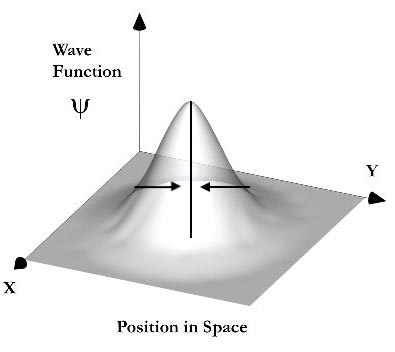
\includegraphics[width=5cm,height=5cm]{Images/eigen-function.jpg}
\caption{Quantum Measurement \cite{noauthor_copenhagen_nodate}}%
\end{figure}
\addcontentsline{toc}{subsubsection}{Figure 6: Quantum Measurement}

In order to obtain a measurable value from the system, the wave function must be collapsed into a specific Eigen function, as can be seen in Figure 6. In quantum mechanics, the possibilities of a wave function are localized into a single particle by adding energy and this localization results in measurement. However, the results from a measurement of the wave function is not random; every Eigen function has a certain probability of occurring. For quantum computing, there is a certain probability of returning 0 and a certain probability of returning 1.

\subsection*{\color{SubSectionBlue}{Quantum Genetic Algorithms}}
\addcontentsline{toc}{subsection}{Quantum Genetic Algorithms} \\

A possible application of quantum computing involves a quantum-genetic algorithm. A standard genetic algorithm is a population-based method which consists of 5 crucial components: initialization of a population, evaluation, parent selection mechanism, variation operators, and survivor selection \cite{garg_vector_2017}. 

\begin{algorithm}
\caption{Standard Genetic Algorithm}
\begin{algorithmic}[1]
\State $t \gets 0$
\State $f(x) \gets \text{Evaluation function}$
\State $population \gets \text{Initial Population}$
\While{$generation < \text{final generation}$}
        \State $values \gets f(population\text)$
        \State $survivors \gets \text{max(}values\text{)}$
        \For{$individual \in survivors$}
            \State $\text{Mutate the Survivors}$
            \State $population \gets \text{Survivor Offsprings}$
        \EndFor
        \State $generation += 1$
\EndWhile
\end{algorithmic}
\end{algorithm}

\addcontentsline{toc}{subsubsection}{Algorithm 1: Standard Genetic Algorithm}

Throughout the course of Algorithm 1, the population should “evolve'' towards an optimal solution. Although genetic algorithms are a good way to optimize problems, classical computers require additional steps in order to mutate the population. Genetic operators such as crossover probability and mutation effects have to be explicitly defined for the population to mutate. On top of that, these genetic operators require hyper parameter turning and will not accurately represent the random variability in most populations. 

\vspace{1mm}

When applied to quantum mechanics, however, previous research has indicated that a quantum genetic algorithm can be used based upon the concepts of quantum bits and quantum superposition states. Using qubit encoding, where each qubit uses a vector to represent binary code, a quantum algorithm can use a quantum system with multiple qubit vectors as an initial population \cite{wu_improvement_2013}. Specifically, each quantum gene is represented by a qubit vector, each quantum chromosome is represented by a bra vector, and each quantum population is represented by a column of chromosomes. When the quantum population is first created, each vector is initialized with a linear superposition of states, essentially setting both $\alpha$ and $\beta$ to  $\sqrt{2} / 2$ , so that the probability of getting a 0 or a 1 during measurement is the same.

\vspace{1mm}

Once the initialization of the population has been completed, the entire quantum population is measured. Measurement involves the evaluation of each individual in the population, as explained in Algorithm 1. However, the evaluation function will differ tremendously depending on the application of the quantum genetic algorithm. The qubit string which produces the highest profit while remaining under the constricting value is stored as the best individual in that generation. The fitness of the best population is then plotted on a curve for future use. In order to create a new generation from the existing quantum population, each qubit’s probability amplitudes are manipulated by a constant (a hyperparameter in the algorithm). When a new generation is created, the inherent randomness of quantum computing is utilized since this randomness creates natural variability in the population. The population will eventually reach a local maximum and the evolutionary algorithm is terminated \cite{nowotniak_higher-order_2014}. Thus, the theory of the genetic algorithm remains the same but a QIGA manipulates qubit vectors, instead of classical values, to create increase optimization.  Higher-Order quantum genetic algorithms use quantum registers to handle the encoding instead of isolated qubit vectors \cite{nowotniak_higher-order_2014}.

\subsection*{\color{SubSectionBlue}{Disaster Algorithm}}
\addcontentsline{toc}{subsection}{Disaster Algorithm} \\

The current setup of the quantum genetic algorithm does not account for the stabilization that occurs when an environment reaches a local optimum. A local optimum is when the genetic algorithm prematurely converges onto a single value for a certain period of time giving the illusion that the absolute maxima, or extremity point has been determined \cite{nowotniak_higher-order_2014}. So, one caveat of the genetic algorithm is the time of convergence in later states of the algorithm. 

\vspace{1mm}

Fu et al. \cite{wu_improvement_2013} addressed this issue and improved local search performance by implementing a self-adaptive rotating angle strategy and a disaster algorithm \cite{wu_improvement_2013}.  The rotating strategy exploited different concepts of linear algebra to decrease the number of parents with each call of the algorithm. The disaster condition, however, imposed a self-made disaster once the genetic algorithm reached a premature convergence value. For example, in some functions, there are various relative maxima and the genetic algorithm might mistake a relative maximum for an absolute maximum. In a quantum system, the disaster was usually resetting the probability amplitudes of some vectors to a linear superposition of states. This prevents premature convergence and ensures that the highest value for the knapsack function is returned.

\vspace{1mm}

Although Fu et al. \cite{wu_improvement_2013} did not test their algorithm using the knapsack problem, their method required similar computational abilities. After testing, researchers concluded that the addition of the rotating technique and the disaster condition improved the times of convergence of the quantum-inspired genetic algorithm, and returned a higher optimization value \cite{wu_improvement_2013}. However, the research that was performed by this team used isolated qubit vectors to encode qubit strings, as common with QIGA algorithms, and the simplicity of the design could have caused a lower optimization value than initially expected.

\subsection*{\color{SubSectionBlue}{Uniqueness of This Researcher's Current Work}}
\addcontentsline{toc}{subsection}{Uniqueness of This Researcher's Current Work} \\

The new research performed addresses the flaws in previous research and allows for greater theoretical optimization of the knapsack problem. In this new algorithm, Quantum Save, the higher-order quantum genetic algorithm is implemented on the IBM Q32 simulator which allows the algorithm to better simulate a quantum state. Quantum Save uses the increased complexity of the Q32 simulator to better mimic the random variations that occur in a genetic algorithm. In addition to that, although Kucharski and Nowotniak \cite{nowotniak_higher-order_2014} provided a range for the amount of probability amplitude manipulation, they didn’t provide a certain value. So, Quantum Save will consist of tuned hyper parameters for which the optimization of the Knapsack problem is the greatest. Also, with Quantum Save, a disaster condition will be added to the higher-order QGA to prevent premature convergence. In fact, social disasters technique, which applies a catastrophic operator once a local maximum is reached is one of the best methods to obtain the global extremity point instead of the local maxima \cite{rocha_preventing_1999}. In Quantum save, the disaster condition will implement a simple quantum catastrophe operator. Therefore, by tuning the higher-ordered QIGA, the probability of reaching a global maximum will increase drastically, and the optimization value for the knapsack problem will be much higher.

In addition to that, Quantum Save can help hospitals and defense contractors save millions by allocating the budgets of small and medium sized targets. In previous research, the cyber security investment model was based upon simulated values and game theory. And with the existing optimization models, like the one proposed by Rakes et al. \cite{rakes_it_2012}, the model performs significantly better for bigger targets since there is more budget to work with. The model does not face the full effect of the budget constraint and can easily choose countermeasures to maximize mitigation. However, it is the smaller-medium sized targets who are the most vulnerable to malware from adversaries. So, Quantum Save uses threat factors and mitigation values from real-life case studies to improve the budget allocation of these small-medium sized targets. Specifically, the data set compiled by Rakes et al. \cite{rakes_it_2012} in Figure 3 is inputted into the quantum algorithm. Researching this topic will allow the scientific and engineering community to accomplish countless tasks that have a limitation factor and an optimization value. Quantum Save can also improve the cybersecurity defenses of hospitals and defense contractors. \\

